%%%%%%%%%%%%%%%%%%%%%%%%%%%%%%%%%%%%%%%%%%%%%%%%%%%%%%%%%%%%%%%%%%%
%
% This is a general template file for the LaTeX package SVJour3
% for Springer journals.          Springer Heidelberg 2010/09/16
%
% Copy it to a new file with a new name and use it as the basis
% for your article. Delete % signs as needed.
%
% This template includes a few options for different layouts and
% content for various journals. Please consult a previous issue of
% your journal as needed.
%
%%%%%%%%%%%%%%%%%%%%%%%%%%%%%%%%%%%%%%%%%%%%%%%%%%%%%%%%%%%%%%%%%%%
%
\RequirePackage{fix-cm}
%
\documentclass[twocolumn]{svjour3}           % twocolumn
%
\smartqed % flush right qed marks, e.g. at end of proof
%
\usepackage{graphicx}
\usepackage{hyperref}
\usepackage[round, sort&compress, numbers]{natbib}
%
\DeclareRobustCommand\IPCClongname{}
%
% please place your own definitions here and don't use \def but
% \newcommand{}{}
%
% Insert the name of "your journal" with
% \journalname{myjournal}
%
\begin{document}

\title{Evaluating the performance  and energy efficiency of COSMO-ART,
  a fully online coupled model  system composed of a numerical weather
  forecast model  and a  chemical transport model.   \thanks{Grants or
    other notes  about the  article that should  go on the  front page
    should be placed here.}}
%\subtitle{Write here subtitle}

%\titlerunning{Short form of title} % if too long for running head

\author{J.Charles \and W.Sawyer \and M.Dolz \and C.Malossi}

%\authorrunning{Short form of author list} % if too long for running
%head

\institute{Dr. Joseph Charles \at Swiss National Supercomputing Centre
  (CSCS)\\ CH-6900  Lugano, Switzerland  \\ Tel: +41  (0) 91  610 8216
  \\ \email{joseph.charles@cscs.ch} \and Dr.  William Sawyer \at Swiss
  National Supercomputing Centre  (CSCS)\\ CH-6900 Lugano, Switzerland
  \\ Tel:  +41 (0) 91 610 8229  \\ \email{william.sawyer@cscs.ch} \and
  Dr.  Manuel Dolz \at University of Hamburg \\ 20148 Hamburg, Germany
  \\         Tel:         +49         (0)        40         460094-404
  \\ \email{manuel.dolz@informatik.uni-hamburg.de}  \and Dr. Cristiano
  Malossi  \at  IBM  Zurich  Research Laboratory  \\  CH-8000  Zurich,
  Switzerland     \\     Tel:      +41     (0)     44     724     8616
  \\ \email{ACM@zurich.ibm.com}}

\date{Received: date / Accepted: date} % The correct dates will be
                                       % entered by the editor

\maketitle

\begin{abstract}
  In this paper we present  COSMO-ART, an extension of the operational
  weather  forecast  model  of   the  German  Weather  Service  (DWD),
  developed for  the evaluation of the interactions  of reactive gases
  and aerosol particles  with the state of atmosphere  at the regional
  scale. It  includes secondary aerosols,  directly emitted components
  like  soot,  mineral  dust,  sea  salt and  biological  material  as
  pollen. Processes such  as emissions, coagulation, condensation, dry
  deposition,  wet removal,  and sedimentation  of aerosols  are taken
  into account.   The overall performance  of this application  on HPC
  systems is  analysed by a  profiling and tracing study  to determine
  hotspots  and  identify   critical  paths.   Moreover,  we  describe
  measurement devices and energy-aware techniques employed to evaluate
  the  energy  footprint of  the  considered  application  and to  get
  detailed  insights about  power bottlenecks.   Our motivation  is to
  improve  corresponding  code sections  to  sustain high  performance
  while  minimizing energy-to-solution.   This preliminary  study sets
  the basis of subsequent  considerations to tackle challenges related
  to energy  efficient high performance computing in  the framework of
  the Exa2Green project (\url{http://exa2green.eu/}).

\keywords{High performance computing  \and Energy-aware computing \and
  Green computing  \and Numerical weather  prediction \and Atmospheric
  chemistry  \and  Aerosols  modelling  \and  Profiling  methods  \and
  Benchmark analysis \and COSMO-ART coupled model}
% \PACS{PACS code1 \and PACS code2 \and more}
% \subclass{MSC code1 \and MSC code2 \and more}
\end{abstract}

\section{Introduction}
\label{intro}
While anthropogenic greenhouse gas emissions are driving unprecedented
major  climate  changes  since   the  mid-20$^{th}$  Century,  one  factor
overwhelmingly  affects  the  uncertainty  in  determining  human-induced
radiative  forcing:  the  effects   of  aerosols  in  the  atmosphere.
Although they  are not considered  heat-trapping greenhouse  gases and
have  shorter  atmospheric lifetimes,  aerosols  significantly modify  the
global   radiation   budget   \citep{IPCC-2013}.   Enhanced   aerosols
concentrations impact the climate  system by scattering and absorption
of solar radiation, thereby exerting a direct radiative forcing; or by
modifying cloud  properties,  cloud  fraction and  surface
albedo,  causing  a  negative  indirect  radiative  forcing.   Despite
considerable  progress in  global aerosol  modelling \citep{Mann-2013}
and  measurement-based  assessments,  large  uncertainties  remain  in
current  estimates  of  aerosol radiative  forcing  \citep{Myhre-2013,
IPCC-2013,  Lee-2013,   Randles-2013,  Rosenfeld-2013,  Sherwood-2013,
Stier-2013}.

Hence to  improve our understanding of  aerosol-cloud interactions and
reduce  these  uncertainties,  the  research  community  is  making  a
concerted international  effort to represent  the underlying physical,
chemical  and aerosol dynamical  processes through  numerical chemical
transport  models (CTMs)  such  as ART  (Aerosols  and Reactive  Trace
gases),   developed   at  the   Karlsruhe   Institute  of   Technology
(KIT)  \citep{Vogel-2009,  Bangert-2011,  Knote-2013}.  This  regional
scale modelling system is coupled  with the operational  weather forecast
model  \textsc{Cosmo}  \citep{Baldauf-2011},  jointly developed and used by  a
consortium of European weather centers, as well as utilised in a climate version
by the wider research community.

The extended  atmospheric model \textsc{Cosmo-art}  is com\-put\-ationally
much  more  demanding than  \textsc{Cosmo}  since  a  large number  of
additional  tracers and  processes have  to be  considered.   Thus the
model  is currently  severely limited  in terms  of applicability  and
expensive in terms of energy consumption.  Although \textsc{Cosmo} has
recently been ported to GPUs \citep{Gysi-2014, Lapillonne-2014} within
the framework of the  High Performance and High Productivity Computing
(HP2C) Initiative  \citep{HP2C} to optimise it  for computational and
energy efficiency,  significant investments in ART  are still required
to take it  to a similar level.  The  efficiency of \textsc{Cosmo-art}
is being  addressed in the  EU Exa2Green project  \citep{EXA2GREEN} to
deliver a  prototype code, which  provides an energy efficiency  of at
least five times the  baseline value.  Such an implementation would
allow  the  community  to  investigate critical  questions  at  higher
resolution  and   over  longer  periods,   at  reduced  cost   to  the
environment.

This  work is  organized as  follows: in  Sec.~\ref{sec:1} we  give an
overview  of  related  work,   then  in  Sec.~\ref{sec:2}  we  briefly
introduce \textsc{Cosmo-art}  and specify its  technical setup related
to  the investigated  performance and  energy evaluation  methods.  In
Sec.~\ref{sec:3}   we  describe   HPC  platforms,   power  measurement
equipments   and  software  environment   employed  to   conduct  this
benchmarking study.  Sec.~\ref{sec:4}  presents performance and energy
requirements  of the  baseline on  these architectures  and highlights
areas where improvements will be necessary for the subsequent baseline
refactoring.   Finally,  we  conclude in Sec.~\ref{concl} with some 
implications for the Exa2Green project and give an outlook for future
research.


\section{The operational COSMO-ART}
\label{sec:1}
\subsection{Model description}
\label{subsec:1.1}



\subsection{Model setup}
\label{subsec:1.2}
\input{Subsec_1.2:Model_Setup.tex}

\section{Hardware description}
\label{sec:2}

\section{Power measurement systems}
\label{sec:3}

\section{Benchmark results}
\label{sec:4}

\section{Conclusion}
\label{concl}

%\paragraph{Paragraph headings} Use paragraph headings as needed.

%\begin{figure*}
%  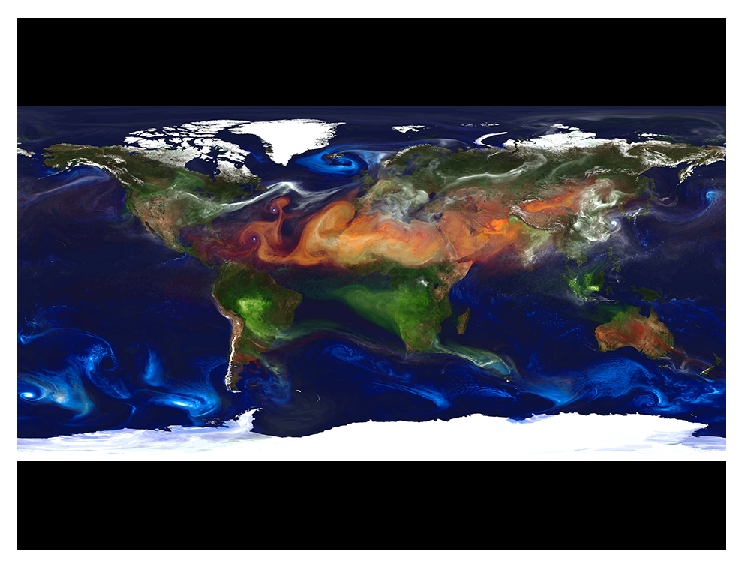
\includegraphics[width=0.4\textwidth]{Figs/earth.eps}
%  \caption{Please write your figure caption here}
%  \label{fig:1}
%\end{figure*}

%\begin{table}
%  \caption{Please write your table caption here}
%  \label{tab:1}
%  \begin{tabular}{lll}
%    \hline\noalign{\smallskip}
%    first & second & third  \\
%    \noalign{\smallskip}\hline\noalign{\smallskip}
%    number & number & number \\
%    number & number & number \\
%    \noalign{\smallskip}\hline
%  \end{tabular}
%\end{table}

\begin{acknowledgements}
This  research  was  supported   by  the  Exa2Green  research  project
co-funded  under the  EU  7th Framework  Program  Future and  Emerging
Technologies (FET) Proactive Initiative: Minimising Energy Consumption
of Computing to  the Limit (MINECC).  The authors  would like to thank
the  High  Performance  and  High  Productivity  Computing  Initiative
(\url{www.hp2c.ch}) for  results that will be  leveraged in subsequent
code refactoring.
\end{acknowledgements}

\DeclareRobustCommand\IPCClongname{ - Intergovernmental Panel on Climate Change}

\bibliographystyle{plainnat}
\bibliography{\jobname}

\end{document}

